% Todo:

\documentclass[12pt]{article}
\usepackage[no-math]{fontspec}	% no-math option required for accents package
\usepackage{hyperref}
\usepackage{xeCJK}
%\setCJKmainfont{SimSun}
\setCJKmainfont[BoldFont=SimHei,ItalicFont=KaiTi]{SimSun}
% \setCJKsansfont{SimHei}
% \setCJKmonofont{SimKai}
\setmainfont{Arial}

\usepackage{accents}		% for dots under Chinese for empahsis
\usepackage{cite}
\usepackage{graphicx}
\usepackage{float}
\usepackage{amsfonts}
% \usepackage{amsmath}	% for \tag
\usepackage{amssymb}	% for \multimap
% \usepackage{stmaryrd}
\usepackage{color}
%\usepackage[square,numbers]{natbib}
%\nocopyright
%\usepackage{latexsym,amsmath,amssymb,graphicx,hyperref}
%\usepackage{times} % gives you a bit more space if needed
\usepackage{titlesec}		% change color of section headings
\usepackage{verbatim}		% enables to define {comment} blocks
%\usepackage[most]{tcolorbox}		% color box

% Left and right angle brackets
\makeatletter
\newsavebox{\@brx}
\newcommand{\llangle}[1][]{\savebox{\@brx}{\(\m@th{#1\langle}\)}%
  \mathopen{\copy\@brx\kern-0.5\wd\@brx\usebox{\@brx}}}
\newcommand{\rrangle}[1][]{\savebox{\@brx}{\(\m@th{#1\rangle}\)}%
  \mathclose{\copy\@brx\kern-0.5\wd\@brx\usebox{\@brx}}}
\makeatother

% Make dots under Chinese characters for emphasis
\renewcommand{\d}[1]{$\underaccent{\scalebox{0.4}{\textbullet}}{\textrm{#1}}$}
\makeatletter\newcommand{\ds}[1]{\@tfor\next:=#1\do{\d{\next}}}\makeatother

\titleformat{\section}
{\color{blue}\normalfont\Large\bfseries}
{\color{blue}\thesection}{1em}{}
\titleformat{\subsection}
{\color{blue}\normalfont\large\bfseries}
{\color{blue}\thesubsection}{1em}{}

\renewcommand\abstractname{\textcolor{blue}{Abstract}}

\definecolor{LogicColor}{rgb}{0.4,0.1,0.4}  % Magenta
\definecolor{Hilight}{rgb}{0.9,0.9,0.8}  % Magenta
% \definecolor{LogicColor}{rgb}{0,0,0}	% for black-and-white paper

\newcommand{\concept}[1]{\textbf{\textcolor{blue}{#1}}}

\newcommand{\english}[1]{\rmfamily \textit{``#1''}\rmfamily}
\newcommand{\formula}[1]{\textcolor{LogicColor}{#1}}

\newcommand{\hilight}[1]{\begin{tcolorbox}[breakable]#1\end{tcolorbox}}

\newcommand{\tab}{\hspace*{1cm}}

\newcommand*\sigmoid{\vcenter{\hbox{
\includegraphics{sigmoid.png}}}}
\newcommand*\sadface{
\includegraphics[scale=0.25]{face-sad.png}}

\setlength{\oddsidemargin}{1cm}
\setlength{\evensidemargin}{1cm}
\setlength{\textwidth}{14cm}

\linespread{1.2}

\title{\textcolor{blue}{Genifer 5.0 理论笔记}}
\author{YKY (\textit{甄景贤})}
%% \date{30 June 2015}
%% \institute{}

\begin{document}

\begin{comment}
\tab\tab\tab \parbox{9cm}{\textit{.....}}
% \vspace{-0.5cm}
\begin{flushright}
\textemdash\, .... \hspace*{2cm}
\end{flushright}
\end{comment}

% \sffamily

{\let\newpage\relax\maketitle}

\maketitle
\setlength{\parindent}{0em}
\setlength{\parskip}{1.5ex plus0.5ex minus1.2ex}

和 Joseph Cheng 谈过之后,我提出进一步简化的新 model:

\section{放弃 sentence structure}

因为太麻烦了,增加了复杂性。  想像一个只能用单字说话的 baby,如果她将来够聪明的话,她可以学会用单字组成句子,但那要视乎她内部知识的增长。 这些语言方面的知识,我们不会 externally program 进去。 宁愿她开始时比较低能,也好过我们 design 到筋疲力尽。

如果 Genifer 只会「出字」,例如听到「妈妈」会输出「喝奶」,那只是很简单的条件反射式动作。 关键是 Genifer 内部有这样的一个 neural reasoner:
\begin{figure}[H]
\centering
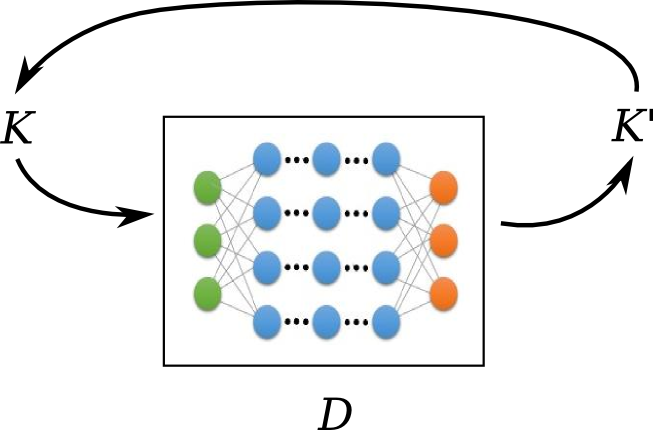
\includegraphics[scale=0.75]{reasoner-model.png}
\end{figure}
它有能力作出多个步骤的推理。

新的 cognitive state vector $K$ 可以是这样的:
\begin{figure}[H]
\centering
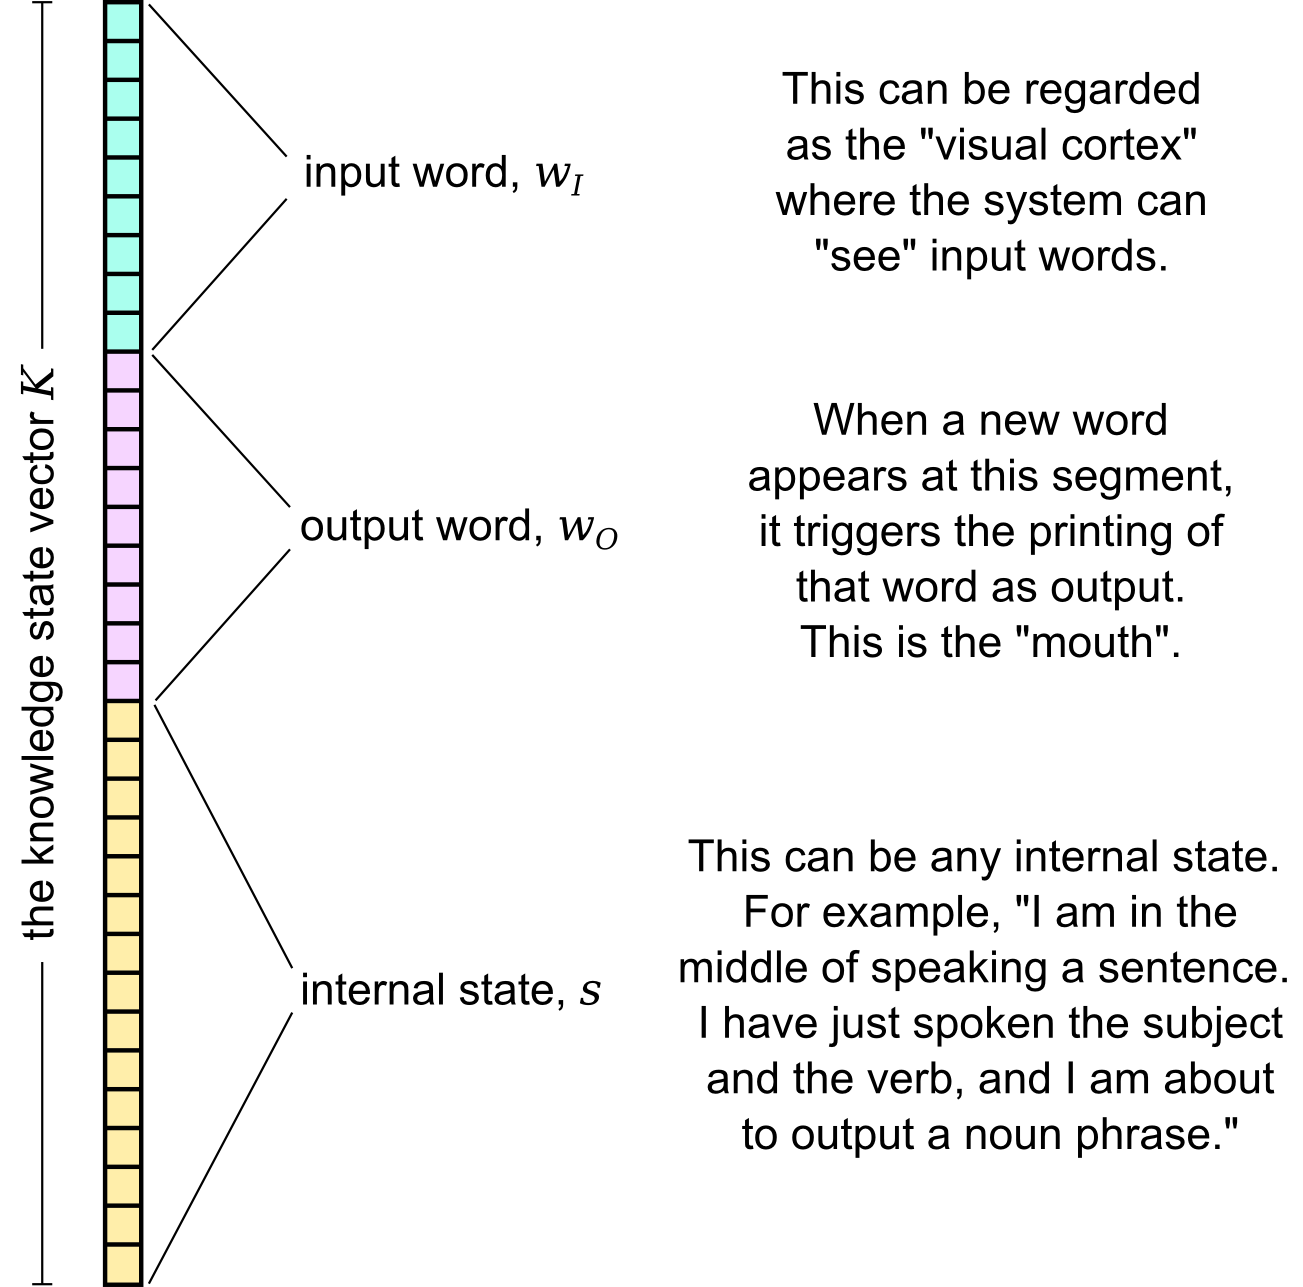
\includegraphics[scale=0.75]{internal-state-K.png}
\end{figure}

$w_I$ 和 $w_O$ 分别是 Genifer 的「眼」和「咀巴」。

$w_I$ 可以是 word2vec 产生的 vector,这里我们只是利用 word2vec 输出的 representation,算法基本上是和 word2vec 无关的。

$w_O$ 是 reasoner 的输出,每当这部分变动时,我们就印出一个新的字。 

$s$ 是「内部状态」,也可以叫 \,"working memory" (认知科学术语),也可以看成是 Turing machine 里的记忆磁带。 它记住当前的问题状态,$D$ 作用在 $K$ 之上,产生新的结论。

{\small 注: 我对中文智能输入法也有兴趣,这里 $w_I$ 可以是键盘字母,$w_O$ 是词语 suggestions 或 auto-complete。}

\section{用 reinforcement learning (RL) 控制 reasoner}

Richard Sutton (强化学习方面的领先研究者)说,RL 应该是人工智能系统的 top-level architecture,我也赞同这点。\footnote{可以参看我在博客上写的 \href{http://geniferology.blogspot.hk/2015/04/what-is-reinforcement-learning.html}{什么是强化学习?}}

整个 Genifer 系统是这样的:
\begin{figure}[H]
\centering
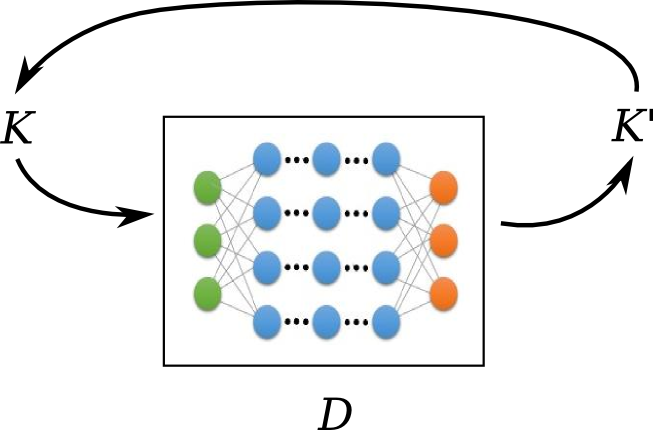
\includegraphics[scale=0.75]{genifer-model-0.png}
\end{figure}

设计一个 RL 系统只需定义 4 个元素: \{ 状态 (states)、行动 (actions)、奖励 (rewards)、方案 (policy) \},其中 policy 是由算法自动计算出来的 states $\rightarrow$ actions 函数。

可以想像 RL 控制一个婴儿慢慢~\ds{调教}她的四肢动作,最后学会走路,这是经典的 RL 应用。

但在 Genifer 中,reasoner 是 Genifer 的一部分,它教导 Genifer 如何思考,但它本身受 RL 控制。

要小心避免 recursive 谬误: 对 RL 来说,reasoner 是一个 external 物体,换句话说,reasoner 虽然是一个导师,但它的内部是\ds{透明的},这个导师本身可以被 RL 调教。

要小心区分 Genifer 的 actions:
\begin{itemize}
\item 她对外部世界的 actions,例如「举手」、「小便」
\item 她对 reasoner 的 \textit{control actions}
\end{itemize}

上次说过,reasoner 只有3个基本动作: 推导、学习、查询。  如果只能调教这3个 actions,则 RL 的作用不大,所以要将 reasoner 的运作「精细化 (refine)」。

方法是: RL 的 control actions 可以直接改写状态 $K$ 的内容。 例如说:『现在紧急状态,要小便』,那么 Genifer 可能会停下现时的工作,去厕所。

$K$ 的内容基本上是无限制的,所以可以有近乎无限的 actions。 在经典 RL 里,通常用一个 table 记录所有 state-action transitions,但在这情况下我们必须用 function approximation 去近似这个 table,这也没有大碍。 

\section{Remaining problems}

\begin{itemize}
\item 查询算法 (query algorithm)
\end{itemize}

\begin{comment}
\section{慢吸 (slow absorption)}

第一个问题是,为什么需要慢慢「吸收」句子?
\begin{itemize}
\item 找出与其他句子的关系
\item 逻辑和谐
\item 找出句子下游的逻辑后果
\item 最后,找出最适当的在句子空间中的位置
\end{itemize}

慢吸需要服从的约束是?
\begin{itemize}
\item fast
\item accurate
\item comprehensive (全面)
\end{itemize}
全面的意思是: 在一定复杂性以下可以推导到的结论,就应该推导到(这涉及 $P =? NP$ 问题)。

现在我们似乎只剩下 $G$ 的结构可以改变。 单单改变 G 是否可以达到「更快、更准、更全面」?

\end{comment}

% \section*{Acknowledgments}

\bibliographystyle{plain} % or number or aaai ...
\bibliography{AGI-book}

\end{document}
